\documentclass[tikz,border=3pt]{standalone}
\usepackage[utf8]{inputenc}
\usepackage[T1]{fontenc}
\usepackage{lmodern}
\renewcommand{\familydefault}{\sfdefault}
\usepackage{sansmath}\sansmath
\usepackage[american]{circuitikz}
\usepackage{pgfplots}\pgfplotsset{compat=1.18,/pgf/number format/use comma,/pgf/number format/1000 sep={.}}
\usetikzlibrary{arrows.meta,calc,positioning,decorations.pathmorphing,patterns}
% paleta del sitio
\definecolor{nar}{HTML}{E8680C}\definecolor{narc}{HTML}{FFB35C}\definecolor{hielo}{HTML}{FFF3E8}
\definecolor{tinta}{HTML}{1D1D1F}\definecolor{gris}{HTML}{6E6E73}\definecolor{lila}{HTML}{7C5CF0}
\definecolor{azul}{HTML}{2F6FD6}\definecolor{menta}{HTML}{17A673}\definecolor{coral}{HTML}{E8342A}
\ctikzset{bipoles/thickness=1.6}
\begin{document}
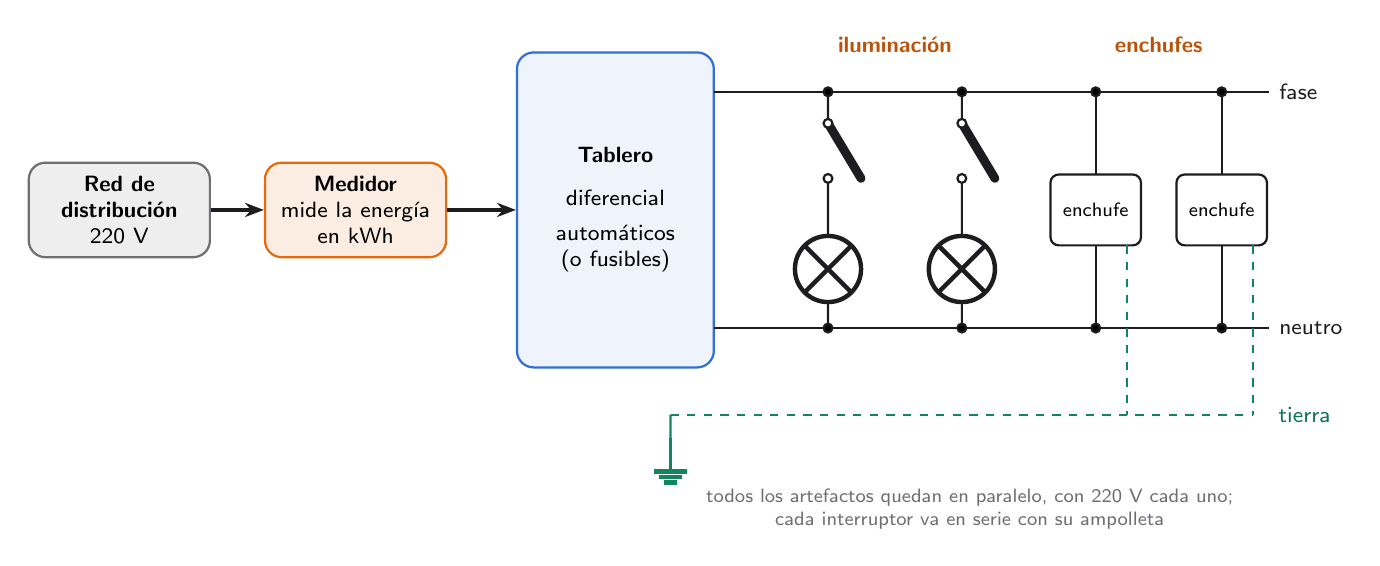
\begin{tikzpicture}[font=\footnotesize,>={Stealth[length=2.4mm]}]
\tikzset{caja/.style={draw=#1,fill=#1!12,thick,rounded corners=6pt,minimum width=2.3cm,minimum height=1.2cm,align=center}}
\node[caja=gris] (R) at (0,2.3) {\textbf{Red de}\\\textbf{distribución}\\220 V};
\node[caja=nar] (M) at (3.0,2.3) {\textbf{Medidor}\\mide la energía\\en kWh};
\node[draw=azul,fill=azul!8,thick,rounded corners=6pt,minimum width=2.5cm,minimum height=4.0cm,align=center] (T) at (6.3,2.3) {\textbf{Tablero}\\[6pt]diferencial\\[3pt]automáticos\\(o fusibles)};
\draw[->,very thick,tinta] (R) -- (M);
\draw[->,very thick,tinta] (M) -- (T);
% fase y neutro
\draw[tinta,thick] (7.55,3.8) -- (14.6,3.8) node[right] {fase};
\draw[tinta,thick] (7.55,0.8) -- (14.6,0.8) node[right] {neutro};
\draw[tinta,thick] (9.0,3.8) to[cosw,*-] (9.0,2.3) to[lamp,-*] (9.0,0.8);
\draw[tinta,thick] (10.7,3.8) to[cosw,*-] (10.7,2.3) to[lamp,-*] (10.7,0.8);
\foreach \x in {12.4,14.0} {
  \draw[tinta,thick] (\x,3.8) node[circ]{} -- (\x,2.75);
  \draw[tinta,thick] (\x,1.85) -- (\x,0.8) node[circ]{};
  \node[draw=tinta,fill=white,thick,rounded corners=3pt,minimum width=1.15cm,minimum height=0.9cm,font=\scriptsize] at (\x,2.3) {enchufe};
  \draw[menta!80!black,thick,dashed] (\x+0.4,1.85) -- (\x+0.4,-0.3);
}
% tierra
\draw[menta!80!black,thick,dashed] (7.0,-0.3) -- (14.4,-0.3);
\draw[menta!80!black,thick] (7.0,-0.3) to[short] (7.0,-0.6) node[ground]{};
\node[text=menta!70!black,anchor=west] at (14.6,-0.3) {tierra};
\node[font=\footnotesize\bfseries,text=nar!80!black] at (9.85,4.4) {iluminación};
\node[font=\footnotesize\bfseries,text=nar!80!black] at (13.2,4.4) {enchufes};
\node[font=\scriptsize,text=gris,align=center] at (10.8,-1.5) {todos los artefactos quedan en paralelo, con 220 V cada uno;\\cada interruptor va en serie con su ampolleta};
\end{tikzpicture}
\end{document}
